\chapter{Posities in 2D}
\label{chapter:positions}

Posities in 2D hebben een x- en een y-co\"ordinaat, net zoals een punt in een grafiek. In Esenthel staat het nulpunt voor het midden van het scherm. Positieve waarden op de X-as staan rechts, negatieve waarden links. Positieve waarden op de Y-as staan bovenaan, negatieve waarden beneden.

\begin{figure}[h]
\centering
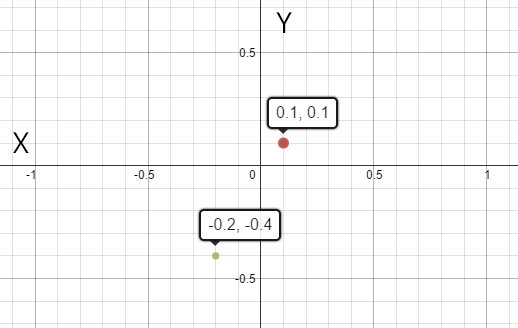
\includegraphics[width=0.7\linewidth]{../images/2Dpositions}
\caption[]{2D co\"ordinaten.}
\label{fig:pos2D}
\end{figure}

In Esenthel gebruiken we de class \texttt{Vec2} om een 2D co\"ordinaat weer te geven. Van een \texttt{Vec2} kan je zowel de x als de y waarde instellen:

\begin{code}
Vec2 pos;
pos.x =  0.1; // de positie op de x-as wordt 0.1
pos.y = -0.3; // de positie op de y-as wordt -0.3
pos   =  0.5; // beide assen krijgen de waarde 0.5
pos.set(0.1, -0.3); // pas beide assen aan via de functie set(float x, float y)
\end{code}

\section{Posities Tonen op het Scherm}

Alhoewel je de class \texttt{Vec2} vooral gebruikt om posities te berekenen, kan je een co\"ordinaat ook op het scherm tonen. Daarvoor bevat de class de functie \texttt{draw(Color)}. Als argument geef je de kleur waarin je je punt wil weergeven. 

\begin{code}
Vec2 p1(0.2, 0.4); // maak een punt p1 en stel x en y in via de constructor.
Vec2 p2;           // maak een punt p2.

void InitPre()
{
   EE_INIT();
}

bool Init()
{
   p2.set(-0.2, -0.5); // stel p2 in via de set functie
   return true;
}

void Shut() {}

bool Update()
{
   if(Kb.bp(KB_ESC)) return false;
   
   return true;
}

void Draw()
{
   D.clear(BLACK); // Maak het scherm leeg
   p1.draw(RED  ); // teken p1 rood  
   p2.draw(BLUE ); // teken p2 blauw
   Vec2(0 ,0).draw(GREEN); // maak een tijdelijk punt en teken dit groen
}

\end{code}

\section{Rekenen}
Je kan met \texttt{Vec2} ook rekenen, net zoals je met getallen doet. Het is mogelijk om de x- en de y-co\"ordinaat afzonderlijk aan te passen, maar je kan ook rechtstreeks rekenen met een \texttt{Vec2}. In dat geval wordt de gekozen berekening voor zowel de x- als de y-as uitgevoerd:

\begin{code}
Vec2 p1(0.1,  0.3);
Vec2 p2(0.3, -0.1);
Vec2 p3 = p1 + p2;  // x: 0.4 , y: 0.2
p3 -= 0.1;          // x: 0.3 , y: 0.1
p3 *= 2;            // x: 0.6 , y: 0.2
p3 = p1 / 2.f;      // x: 0.05, y: 0.15 
\end{code}

\section{Punten om te onthouden}
In Esenthel betekent \texttt{Vec2(0,0)} steeds het midden van het scherm. Maar de randen van het scherm zijn minder duidelijk. Niet elk computerscherm heeft immers hetzelfde formaat. Daarom kan je via het object \texttt{D} (display) de breedte en de hoogte van het scherm opvragen via de functies \texttt{w()} en \texttt{h()}. Zo kan je eenvoudig enkele punten berekenen.

\begin{code}
Vec2 middle(0,0);
Vec2 left(-D.w(), 0);
Vec2 right(D.w(), 0);
Vec2 rightUpperCorner(D.w(), D.h());
Vec2 leftUpperCorner(-D.w(), D.h());
\end{code}

Indien je een punt wil tekenen op afstand 0.1 van de linkerbovenhoek, dan kan je dat dus zo doen:

\begin{code}
Vec2(-D.w() + 0.1, D.h() - 0.1).draw(PINK);
\end{code}

\section{Samengevat}
\begin{itemize}
\item Punten in 2D hebben een x- en een y-co\"ordinaat. In Esenthel gebruik je de class \texttt{Vec2} om een punt weer te geven.
\item De class \texttt{Vec2} heeft een functie \texttt{draw(Color)} om het punt op het scherm te tonen.
\item Je kan rekenen met een \texttt{Vec2}, net zoals met getallen.
\item \texttt{Vec2(0,0)} is steeds het midden van het scherm.
\item De randen van het scherm kan je berekenen via \texttt{D.w()} en \texttt{D.h()}.
\end{itemize}

\section{Oefening}
Maak een programma dat de volgende punten toont:
\begin{enumerate}
	\item Een wit punt in het midden van het scherm.
	\item Een rood punt op afstand 0.1 van de linkerkant van het scherm.
	\item Een blauw punt op afstand 0.2 van de rechterbovenhoek.
	\item Een geel punt op afstand 0.35 van de onderkant van het scherm, op 2/3 van de totale schermbreedte.
\end{enumerate}
